\documentclass{ctexart}  
\usepackage[left=2cm,right=1.97cm,top=2cm,bottom=2cm]{geometry}	
\usepackage{ctex}
\usepackage{palatino}
\usepackage{lipsum}
\usepackage{graphicx}
\usepackage{tabularray}
\usepackage{color}
\usepackage{float}
\title{\heiti \zihao{2}实验一:Git和Latex使用学习实验报告}
\author{\kaishu \zihao{-4} 邓林\qquad 23020007014\\
\songti \zihao{-5}中国海洋大学 \qquad 23软件工程 }
\date{}
\ctexset{section={format={\heiti \zihao{4}}},
subsection={format={ \songti \zihao{4}},beforeskip=0pt,afterskip=0pt},
subsubsection={format={\kaishu \zihao{4}},beforeskip=0pt ,afterskip=0pt}}
%%%%%%%%%%%%%%%%%%%%%%%%%

\begin{document}
    \maketitle
\vspace{-20pt}\begin{abstract}				
    本实验报告主要记录了作者通过课程网站及B站学习Git知识和Latex用法的学习过程以及心得。
\end{abstract}

\section{实验内容}
\subsection{版本控制(Git)}
下载Git,学习Git的命令行接口。克隆课程网站仓库,将版本历史可视化并进行探索,完成课后习题。\\
\subsection{Latex文档编辑}
学习Latex的使用方法,并制作自己的实验报告模板。\\
\vspace{-10pt}\section{操作指令}


\begin{table}[H]
    \centering
   
    \begin{tblr}{
      row{1} = {c},
      cell{1}{1} = {c=2}{},
      cell{2}{1} = {c},
      cell{3}{1} = {c},
      cell{4}{1} = {c},
      cell{5}{1} = {c},
      cell{6}{1} = {c},
      cell{7}{1} = {c},
      cell{8}{1} = {c},
      cell{9}{1} = {c},
      cell{10}{1} = {c},
      cell{11}{1} = {c},
      hline{1-2,12} = {-}{},
    }
    练习用Git命令行                        &                \\
    git init                         & 创建一个新的 git 仓库  \\
    git status                       & 显示当前的仓库状态      \\
    git commit                       & 创建一个新的提交       \\
    git clone                        & 从远端下载仓库        \\
    git log                          & 显示历史日志         \\
    git log --all --graph --decorate & 可视化历史记录(有向无环图) \\
    git branch name                  & 创建分支          \\
    git branch                       & 显示分支           \\
    git remote                       & 列出远端           \\
    git remote add name url          & 添加一个远端         
    \end{tblr} 
    \caption{Git}
    \end{table}

   
    \definecolor{MineShaft}{rgb}{0.2,0.2,0.2}
    \begin{longtblr}[
      label = none,
      entry = none,
    ]{
      row{1} = {c},
      cell{1}{1} = {c=2}{},
      cell{2}{1} = {c},
      cell{3}{1} = {c},
      cell{4}{1} = {c},
      cell{5}{1} = {c},
      cell{6}{1} = {c},
      cell{7}{1} = {c,fg=MineShaft},
      cell{8}{1} = {c},
      cell{9}{1} = {c},
      cell{10}{1} = {c},
      cell{11}{1} = {c,fg=MineShaft},
      cell{12}{1} = {c},
      cell{13}{1} = {c,fg=MineShaft},
      cell{14}{1} = {c,fg=MineShaft},
      cell{15}{1} = {c},
      hlines,
      vlines,
    }
    练习用Latex命令行                                                                                                                                                                                                                                                                                                                                                                                                                                                                                                                                                                                                                                                                                                                                                                                                                                                                                &                                      \\
    \textbackslash{}documentclass\{ctexart\}                                                                                                                                                                                                                                                                                                                                                                                                                                                                                                                                                                                                                                                                                                                                                                                                                                                   & 使用 Latex编写包含中文的文档                    \\
    \textbackslash{}usepackage[leftright,top,bottom]\{geometry\}                                                                                                                                                                                                                                                                                                                                                                                                                                                                                                                                                                                                                                                                                                                                                                                                                               & 设置页边距                                \\
    \textbackslash{}title\{\textbackslash{}heiti \textbackslash{}zihao\{2\}~\%title\}                                                                                                                                                                                                                                                                                                                                                                                                                                                                                                                                                                                                                                                                                                                                                                                                          & 编辑标题字体,字号,内容                         \\
    \textbackslash{}date\{\textbackslash{}today\}\textcolor[rgb]{0.2,0.2,0.2}{}                                                                                                                                                                                                                                                                                                                                                                                                                                                                                                                                                                                                                                                                                                                                                                                                                & 编辑日期                                 \\
    {\textbackslash{}\textcolor[rgb]{0.2,0.2,0.2}{ctexset}\textcolor[rgb]{0.2,0.2,0.2}{\{}\textcolor[rgb]{0.2,0.2,0.2}{section=\{format=\{\textbackslash{}heiti \textbackslash{}zihao\{4\}\}\},}\textcolor[rgb]{0.2,0.2,0.2}{}\\\textcolor[rgb]{0.2,0.2,0.2}{subsection=\{format=\{ }\textcolor[rgb]{0.2,0.2,0.2}{\textbackslash{}}\textcolor[rgb]{0.2,0.2,0.2}{heiti \textbackslash{}zihao\{5\}}\textcolor[rgb]{0.2,0.2,0.2}{\},beforeskip=}\textcolor[rgb]{0.2,0.2,0.2}{0}\textcolor[rgb]{0.2,0.2,0.2}{pt,afterskip=}\textcolor[rgb]{0.2,0.2,0.2}{0}\textcolor[rgb]{0.2,0.2,0.2}{pt\}}\textcolor[rgb]{0.2,0.2,0.2}{,}\textcolor[rgb]{0.2,0.2,0.2}{}\\\textcolor[rgb]{0.2,0.2,0.2}{subsubsection=\{format=\{\textbackslash{}kaishu }\textcolor[rgb]{0.2,0.2,0.2}{\textbackslash{}}\textcolor[rgb]{0.2,0.2,0.2}{zihao\{5\}\},beforeskip=0pt ,afterskip=0pt\}\}}\textcolor[rgb]{0.2,0.2,0.2}{}} & 编辑各级标题字体,字号,行间距                      \\
    \textbackslash{}begin\{document\}\textbackslash{}end\{document\}                                                                                                                                                                                                                                                                                                                                                                                                                                                                                                                                                                                                                                                                                                                                                                                                                           & 编辑文档内容                               \\
    \textbackslash{}vsapce\{10pt\}                                                                                                                                                                                                                                                                                                                                                                                                                                                                                                                                                                                                                                                                                                                                                                                                                                                             & 增加/减少行间距                             \\
    {\textbackslash{}begin\{abstract\}\\\textbackslash{}end\{abstract\}}                                                                                                                                                                                                                                                                                                                                                                                                                                                                                                                                                                                                                                                                                                                                                                                                                       & 编辑摘要                                 \\
    \textbackslash{}maketitle                                                                                                                                                                                                                                                                                                                                                                                                                                                                                                                                                                                                                                                                                                                                                                                                                                                                  & 写入标题                                 \\
    {\textbackslash{}begin\{enumerate\}\\\textbackslash{}item~ 内容~\\\textbackslash{}item 内容\\\textbackslash{}end\{enumerate\}}                                                                                                                                                                                                                                                                                                                                                                                                                                                                                                                                                                                                                                                                                                                                                                 & 段落自动标号                               \\
    url\{~\%链接 \}~                                                                                                                                                                                                                                                                                                                                                                                                                                                                                                                                                                                                                                                                                                                                                                                                                                                                             & 插入超链接                                \\
    {\textbackslash{}begin\{itemize\}\\\textbackslash{}item 内容\\\textbackslash{}item 内容\\\textbackslash{}end\{itemize\}}                                                                                                                                                                                                                                                                                                                                                                                                                                                                                                                                                                                                                                                                                                                                                                       & · 强调符号\textcolor[rgb]{0.2,0.2,0.2}{} \\
    {\textbackslash{}begin\{figure\}{[}htbp]\\\textbackslash{}centering\\\textbackslash{}includegraphics[图片大小]\{图片路径\}\\\textbackslash{}caption\{图片标题、说明\}\\\textbackslash{}label\{fig:图片标签\}\\end\{figure\}}                                                                                                                                                                                                                                                                                                                                                                                                                                                                                                                                                                                                                                                                                  & 插入图片                                 \\
    {\% \textbackslash{}usepackage\{tabularray\}\\\textbackslash{}begin\{table\}{[}h]\\\textbackslash{}end\{table\}\textcolor[rgb]{0.2,0.2,0.2}{}}                                                                                                                                                                                                                                                                                                                                                                                                                                                                                                                                                                                                                                                                                                                                             & 插入表格                                 
    \end{longtblr}
    
\section{练习实例}
\subsection{Git}
\vspace{5pt}\subsubsection{克隆课程网站仓库}
\vspace{5pt}\begin{enumerate}
    \item 获取自己建的ssh密钥信息
\begin{figure}[H]
    \centering
    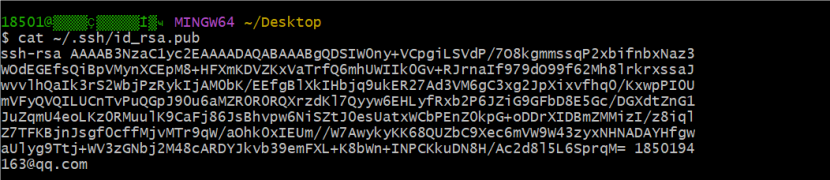
\includegraphics[width=19cm]{111.png}
    \caption{cat\quad\textasciitilde{}/.ssh/id\_rsa.pub}
    \label{fig:11}
\end{figure}
    \item 通过 SSH(安全外壳协议)连接到 GitHub 服务器
     \begin{figure}[H]
        \centering
        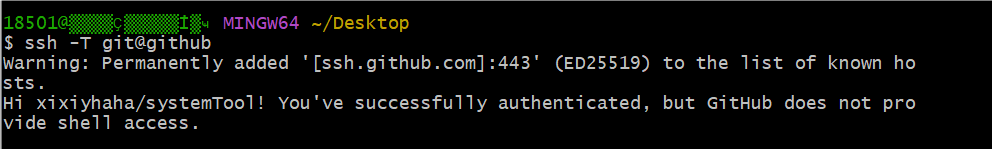
\includegraphics[width=19cm]{3.png}
        \caption{ssh -T git@github.com}
        \label{fig:12}
    \end{figure}
    \item git clone: 克隆仓库
    \begin{figure}[H]
       \centering
       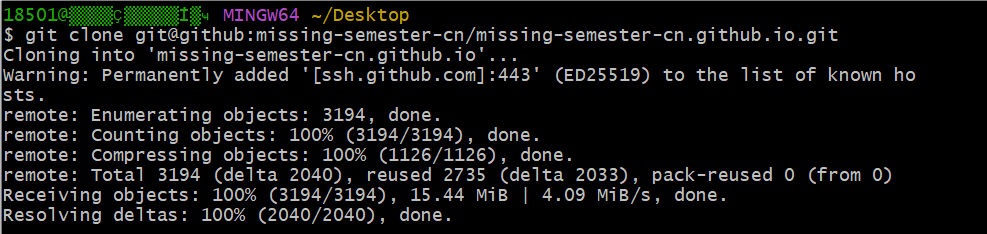
\includegraphics[width=19cm]{4.png}
       \caption{git clone}
       \label{fig:13}
   \end{figure}

\vspace{-5pt}\item git log: 查看历史日志,按q退出
     \begin{figure}[H]
        \centering
        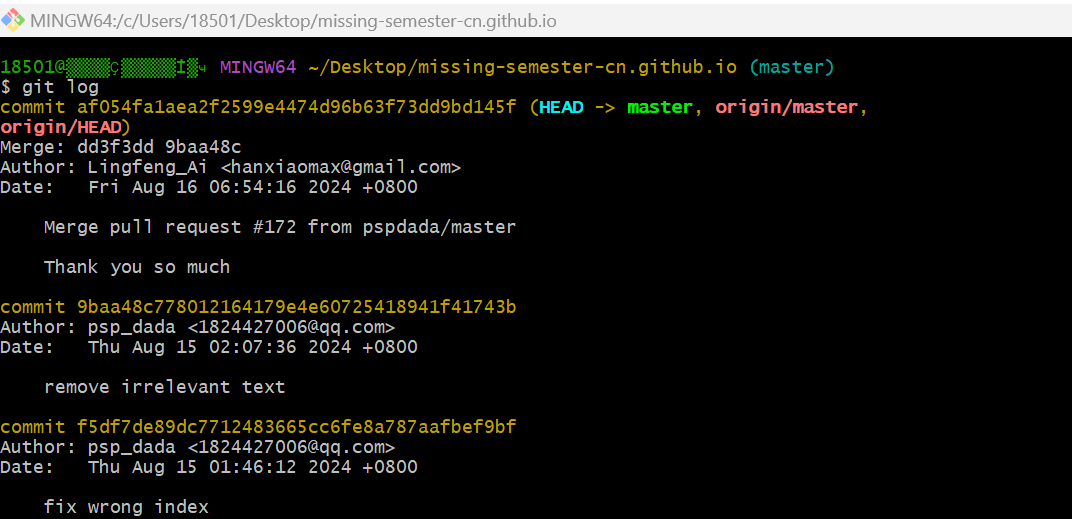
\includegraphics[width=9cm]{5.png}
        \caption{git log}
        \label{fig:14}
    \end{figure}

    \vspace{-5pt}\item git log --all --graph --decorate: 可视化历史记录(有向无环图)
    \begin{figure}[H]
       \centering
       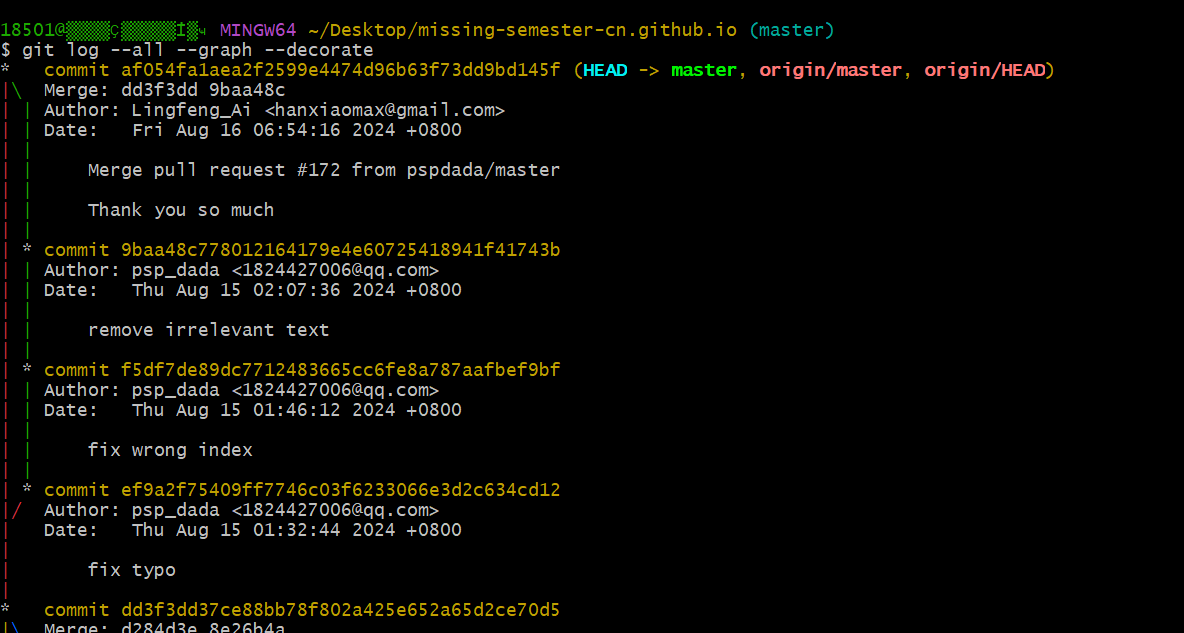
\includegraphics[width=9cm]{6.png}
       \caption{git log --all --graph --decorate}
       \label{fig:15}
   \end{figure}
\end{enumerate}


\subsection{Latex}
使用Latex自己编辑的实验报告模板代码如下:
\begin{figure}[H]
    \centering
    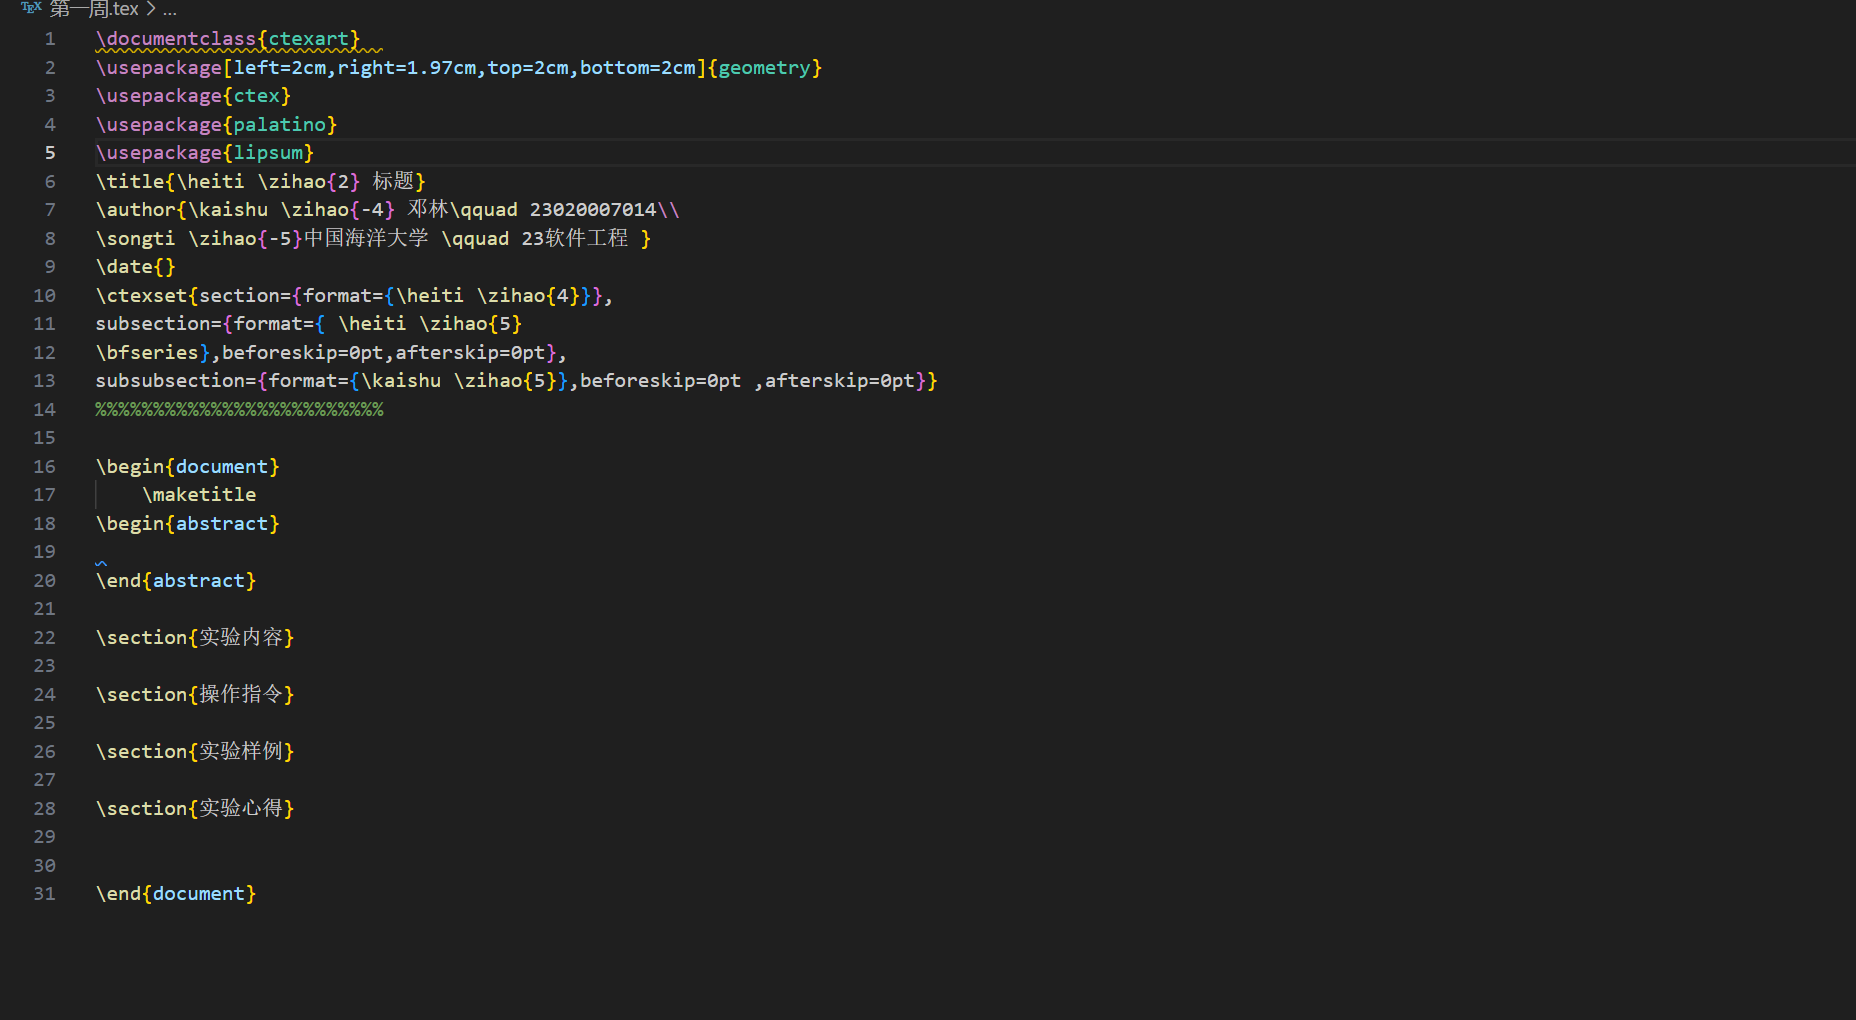
\includegraphics[width=9cm]{20240830000426.png}
    \caption{实验报告模板代码}
    \label{fig:16}
\end{figure}
\section{困难与解决}

\subsection{ssh未连接到Github}
\begin{enumerate}
    \item 通过 SSH(安全外壳协议)连接到 GitHub 服务器\\
    \begin{figure}[H]
        \centering
        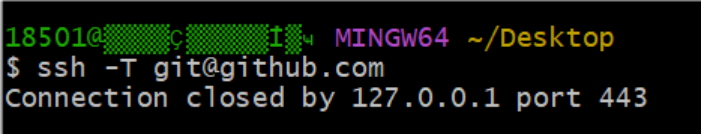
\includegraphics[width=9cm]{image.png}
        \caption{ssh -T git@github.com}
        \label{fig:21}
    \end{figure}
    这里检测发现ssh未连接到GitHub
    \item 打开config文件查看信息,发现有问题
    \begin{figure}[H]
        \centering
        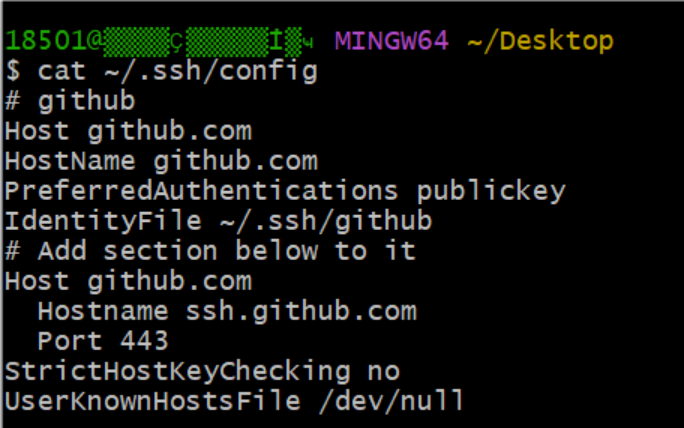
\includegraphics[width=9cm]{image copy.png}
        \caption{cat ~/.ssh/config}
        \label{fig:22}
    \end{figure}
    \item 编辑config文件,添加代码,连接成功
    \begin{figure}[H]
        \centering
        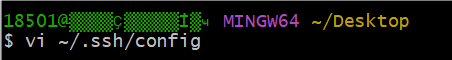
\includegraphics[width=9cm]{1.png}
        \caption{vi ~/.ssh/config}
        \label{fig:23}
    \end{figure}
    \begin{figure}[htbp]
        \centering
        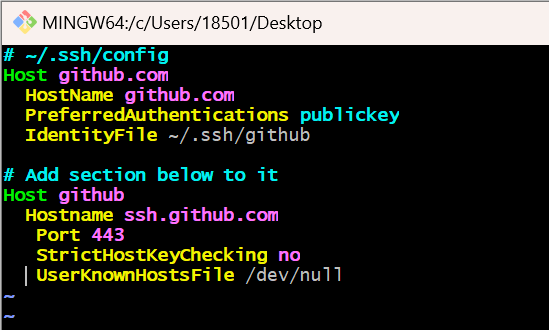
\includegraphics[width=9cm]{2.png}
        \caption{vi ~/.ssh/config}
        \label{fig:24}
    \end{figure}
\end{enumerate}

\subsection{使用 git clone + 仓库ssh协议网址,报错}

    1. 尝试使用 SSH 协议克隆 GitHub 仓库时遇到了 "Connection refused" 错误。这是因为在 .ssh/config 文件中配置了 GitHub 的 SSH 连接使用非标准端口 443,而 git clone 命令默认使用端口 22。
    \begin{figure}[htbp]
        \centering
        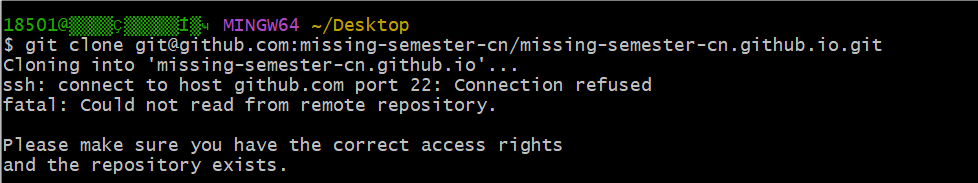
\includegraphics[width=9cm]{7.png}
        \caption{}
        \label{fig:25}
    \end{figure}
    可更改为使用 github 标签来连接到 GitHub
    \begin{figure}[htbp]
        \centering
        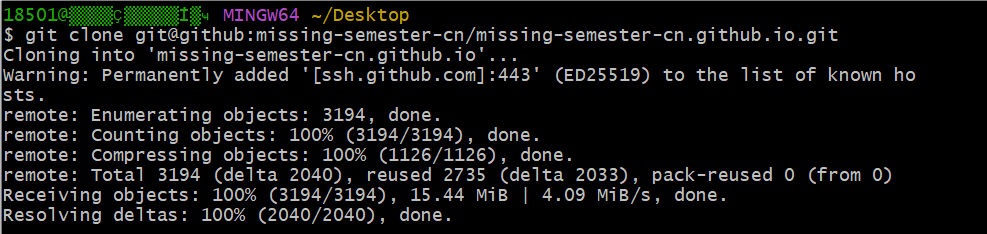
\includegraphics[width=9cm]{8.png}
        \caption{}
        \label{fig:26}
    \end{figure}
    \par2. 也可以修改文件
    \begin{figure}[htbp]
        \centering
        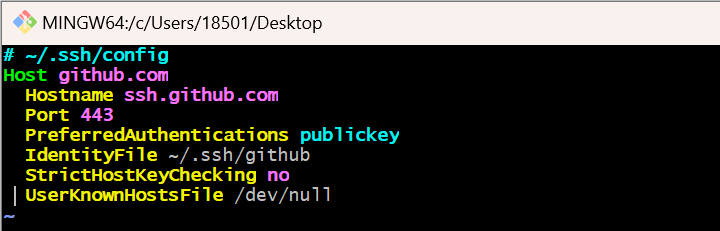
\includegraphics[width=9cm]{9.png}
        \caption{}
        \label{fig:27}
    \end{figure}
    ,用git@github.com 连接:
    \begin{figure}[H]
        \centering
        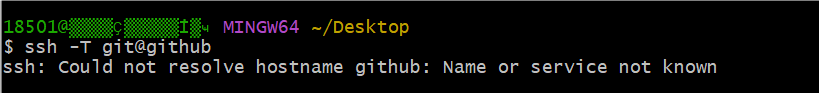
\includegraphics[width=9cm]{10.png}
        \caption{}
        \label{fig:28}
    \end{figure}
    \begin{figure}[htbp]
        \centering
        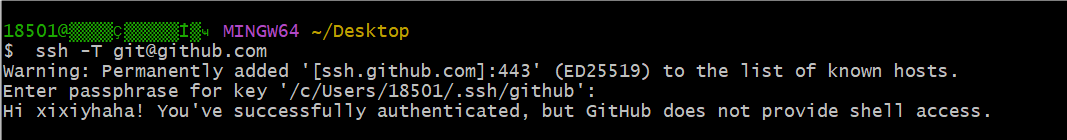
\includegraphics[width=9cm]{11.png}
        \caption{}
        \label{fig:28}
    \end{figure}
    \begin{figure}[htbp]
        \centering
        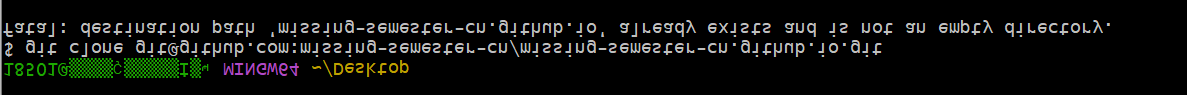
\includegraphics[width=9cm]{12.png}
        \caption{}
        \label{fig:28}
    \end{figure}

\section{实验心得}
    \subsection{Git}
    本次Git学习遇到了许多困难,其中最大的问题就是我的ssh密钥配置有很多的问题,但因为
    对Git方面的知识十分不了解,所以看不懂错误提示,也完全不知道如何下手去解决问题。
    因此只能上网查资料或者看课程资料,但种类繁多,筛选信息也十分困难。最终通过询问同学,
    使用人工智能,才逐步了解这些知识,最终解决。
    \subsection{Latex}
    本次Latex学习相较于Git,体验较为轻松。在网上能学习到比较系统的安装、配置Latex操作系统
    的视频,以及使用教程。学习的方向更加明确,学习起来也就更加轻松。掌握了一些基本的编写
    操作,如标题,分级章节,插入图片、表格、链接等等。我也在学习的过程中体会到了Latxe文本编辑器
    的便捷之处,也更加让我有了使用该系统代替word的想法,虽然图片位置调整仍觉得十分困难。

\end{document}